\documentclass{article}
\usepackage{multicol}
\usepackage{amsmath,mathrsfs,amsfonts}
\usepackage{tikz}
\usetikzlibrary{arrows,shapes,chains}
\usepackage{flowchart}
\usepackage{xcolor}
\usepackage{setspace}
\usepackage{CJK}
\usepackage{geometry}
\usepackage{graphicx}
\usepackage{caption}
\usepackage{float,subfigure}
\geometry{a4paper,scale=0.8}
\usepackage[colorlinks,linkcolor=blue]{hyperref}
\hypersetup{CJKbookmarks=true}
\usepackage{parskip}
\setlength{\parindent}{0cm}

%分一行.
\newcommand{\onech}[4]{
\vspace{-3pt}
\indent
\hspace{16.5pt}
\makebox[101pt][l]{(A) #1} \hfill
\makebox[101pt][l]{(B) #2} \hfill
\makebox[101pt][l]{(C) #3} \hfill
\makebox[101pt][l]{(D) #4}\\
\vspace{-5pt}}
%分两行.
\newcommand{\twoch}[4]{
\vspace{-3pt}
\indent
\makebox[110pt][l]{\qquad(A) #1} \hfill
\makebox[220pt][l]{(B) #2}\\
\indent
\makebox[110pt][l]{\qquad(C) #3} \hfill
\makebox[220pt][l]{(D) #4}\\
\vspace{-5pt}}
%分四行.
\newcommand{\fourch}[4]{
\vspace{-3pt}
\indent\makebox[262pt][l]{\qquad(A) #1}\\
\indent\makebox[262pt][l]{\qquad(B) #2}\\
\indent\makebox[262pt][l]{\qquad(C) #3}\\
\indent\makebox[262pt][l]{\qquad(D) #4}\\
\vspace{-5pt}}

\begin{document}
\begin{spacing}{1.4}
\begin{CJK}{UTF8}{gbsn}
\author{试卷来源:295356805(QQ群)\hspace{1cm}试卷提供:杳思思\hspace{.3cm}风颜\hspace{1cm}排版:回眸人}
\title{2018华科824信号与系统}
\maketitle


\section{选择题}

1、关于信号$\delta(t)$,以下说法错误的是(\hspace{1cm})

\onech{因果信号}{有限带宽}{能量有限}{绝对可积}

2、对于系统
$y(t)=
\begin{cases}
0&,x(t)<0\\
x(t)+x(t-1)&,x(t)\geq 0
\end{cases}$
,下列说法正确的是(\hspace{1cm})

\onech{可逆系统}{无记忆系统}{线性系统}{时不变系统}

3、当$n<1$时,有$c[n]=0$的是(\hspace{1cm})

\twoch{$c[n]=u[n-1]*u[n]$}
{$c[n]=\{u[n+1]-u[n-1]\}*u[n]$}
{$c[n]=u[-n-1]*2^nu[-n]$}
{$c[n]=\delta[n]*2^{-n}u[n]$}

4、积分器的单位冲激响应是(\hspace{1cm})

\onech{$u(t)$}{$tu(t)$}{$\delta(t)$}{$\delta '(t)$}

5、$x(t)=\displaystyle\frac{sin10\pi t}{\pi t}$,则以下哪个带宽最大(\hspace{1cm})

\onech{$x^2(t)$}{$x(3t)$}{$x(t)*x(t)$}{$\displaystyle x(\frac{t}{2})$}

6、信号$[\displaystyle cos(4t-\frac{2}{3}\pi)]^2$的最小正周期为(\hspace{1cm})

\onech{$\displaystyle \frac{\pi}{2}$}{$\displaystyle \frac{\pi}{8}$}{$\displaystyle \frac{\pi}{4}$}{$\pi$}

7、以下说法正确的是(\hspace{1cm})

\fourch
{纯虚奇函数的傅里叶变换也是纯虚奇函数}
{奇函数的傅里叶变换与偶函数的傅里叶变换的卷积也是奇函数}
{$u(\omega)-u(\omega-2)$的时域信号为实信号}
{$sin\omega\cdot cos2\omega$的时域信号是实奇信号}

8、信号$y[n]-2y[n-1]+y[n-2]=2x[n]-x[n-1]$的自由响应模式为(\hspace{1cm})

\onech{$C_1n^2+C_2n+C_3$}{$C_1n$}{$C_1n+C_2$}{$C_1n^2$}

9、系统函数为$H(s)=\displaystyle\frac{s+1}{s^2+2s+2}$的因果LTI系统,当输入为$e^{-|t|}$时,输出信号的收敛域为(\hspace{1cm})

\onech{$Re\{s\}>-1$}{$Re\{s\}<1$}{$Re\{s\}>1$}{$-1<Re\{s\}<1$}

10、$x(t)$为偶信号,且$X(s)$存在一极点$p=-1+2j$,则下列哪个一定是$X(s)$的极点(\hspace{1cm})

\onech{$0$}{$1-2j$}{$-1$}{$-1-2j$}





\section{填空题}

1、对于离散信号$x[n]=cos(\displaystyle\frac{3\pi}{2}n)+sin(\displaystyle\frac{3\pi}{4}n)$,其周期为\underline{\hbox to 20mm{}},平均功率为\underline{\hbox to 20mm{}},

\hspace{15pt}在周期$(-\pi,\pi]$上的傅里叶变换为\underline{\hbox to 20mm{}}.
\vspace{10pt}

2、对于信号$x(t)=\begin{cases}1&,|t|<1\\0&,1<|t|<4\end{cases}$,周期为8,其指数型傅里叶级数为\underline{\hbox to 20mm{}};

\hspace{15pt}化为三角型傅里叶级数有$a_0+2\displaystyle\sum_{k=1}^{\infty}A_kcos(\frac{k\pi}{4}t+\phi_k)$,$A_5$=\underline{\hbox to 20mm{}}.
\vspace{10pt}

3、$x[n]=cos[\displaystyle\frac{\pi}{2}(n^2-2n+1)]^2\cdot\delta[n-1]$的化简形式为\underline{\hbox to 20mm{}};

\hspace{15pt}Z变换为\underline{\hbox to 20mm{}},收敛域为\underline{\hbox to 20mm{}}.
\vspace{10pt}

4、单边拉氏变换$X(s)=\displaystyle\frac{1}{1+e^{-2s}}$,其收敛域为\underline{\hbox to 20mm{}},逆变换$x(t)=$\underline{\hbox to 20mm{}}.
\vspace{10pt}





\section{解答题}

1、已知$x(-2t+1)$的图形如下,画出$x(2t+1)$的图形,并进一步画出$x(t)$的图形(进行必要的标注).

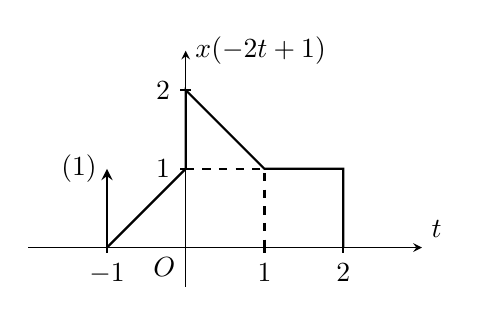
\begin{tikzpicture}[auto,>=stealth,thick]
\draw[->,thin](-2,0)--(3,0) node[above right]{$t$};
\draw[->,thin](0,-.5)--(0,2.5) node[right]{$x(-2t+1)$};
\draw[->](-1,0)--(-1,1) node[left]{$(1)$};
\draw[-](-1,0)--(0,1)--(0,2)--(1,1)--(2,1)--(2,0){};
\draw[-,dashed](0,1)--(1,1)--(1,0){};
\draw[shift={(0,0)}](0pt,0pt)--(0pt,0pt) node[below left]{$O$};
\foreach \x/\xtext in {-1/-1,1/1,2/2}
  \draw[shift={(\x,0)}] (0pt,2pt) -- (0pt,-2pt) node[below]{$\xtext$};
\foreach \y/\ytext in {1/1,2/2}
  \draw[shift={(0,\y)}] (2pt,0pt) -- (-2pt,0pt) node[left]{$\ytext$};
\end{tikzpicture}

\pagebreak



2、系统如图,其中
$x(t)=cos(500\pi t)$,
$p(t)=\displaystyle\sum_{n=-\infty}^{+\infty}\delta(t-\frac{2\pi n}{\omega_s})$,
$H_L(j\omega)=\begin{cases}\displaystyle\frac{2\pi}{\omega_s}&,|\omega|<\displaystyle\frac{\omega_s}{2}\\0&,other\end{cases}$,

\vspace{-15pt}
\begin{minipage}{0.5\textwidth}
\setlength{\parindent}{2em}
(1)求$X(j\omega)$,$P(j\omega)$,并画频谱图;

(2)当$\omega_s=1500\pi$时,求$r(t)$;

(3)当$\omega_s=800\pi$时,求$r(t)$.
\setlength{\parindent}{0em}
\end{minipage}
\begin{minipage}{0.5\textwidth}
\vspace{10pt}
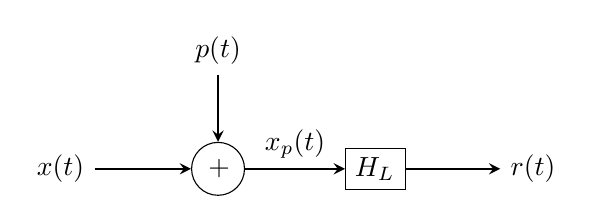
\begin{tikzpicture}[>=stealth,thick]
  \tikzstyle{mul}=[circle,draw,thin,fill=white,text width=.7em]
  \tikzstyle{sys}=[rectangle,draw,thin,fill=white,text width=1.5em]
  \node(x-in) at (0,0)[]{$x(t)$};
  \node(p-t) at (2,1.5)[]{$p(t)$};
  \node(mul) at (2,0)[mul]{$+$};
  \node(sys) at (4,0)[sys]{$H_L$};
  \node(r-out) at (6,0)[]{$r(t)$};
  \draw[->](x-in)--(mul);
  \draw[->](p-t)--(mul);
  \draw[->](mul)--node[above]{$x_p(t)$}(sys);
  \draw[->](sys)--(r-out);
\end{tikzpicture}
\end{minipage}

\vspace{8cm}



3、因果系统$H(z)=\displaystyle\frac{z^{-1}-2z^{-2}}{1-0.5z^{-1}},|z|>0.5$,

\setlength{\parindent}{2em}
(1)画出零极点图;

(2)通过频率响应说明该系统是全通系统;

(3)求$h[n]$;

(4)当输入为$\displaystyle x[n]=1+sin(\frac{\pi}{2}n)+cos(\frac{\pi}{2}n)$时,求$y[n]$.
\setlength{\parindent}{0em}

\pagebreak



4、因果系统框图如图,$a,b,c$均为实系数,已知当输入为$x(t)=u(t)$时,全响应为$y(t)=[1-e^{-t}+3e^{-3t}]u(t)$,

\vspace{-30pt}
\begin{minipage}{.3\textwidth}
\setlength{\parindent}{2em}
(1)求$a,b,c,H(s)$及收敛域;

(2)求$y_{zs}(t)$及$y_{zi}(t)$;

(3)求$y(0^-)$和$y'(0^-)$.
\setlength{\parindent}{0em}
\end{minipage}
\begin{minipage}{.7\textwidth}
\vspace{40pt}
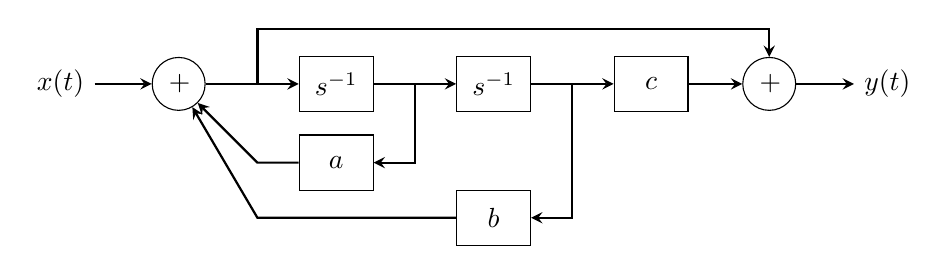
\begin{tikzpicture}[auto,>=stealth,thick]
\tikzstyle{add}=[circle,draw,thin,fill=white,text width=.7em]
\tikzstyle{sys}=[rectangle,draw,thin,fill=white,minimum width = 1em, minimum height=2em,text width=2em,text centered]
\node(x-in)at(0,0)[]{$x(t)$};
\node(add1)at(1.5,0)[add]{$+$};
\node(int1)at(3.5,0)[sys]{$s^{-1}$};
\node(int2)at(5.5,0)[sys]{$s^{-1}$};
\node(c)at(7.5,0)[sys]{$c$};
\node(add2)at(9,0)[add]{$+$};
\node(y-out)at(10.5,0)[]{$y(t)$};
\node(a)at(3.5,-1)[sys]{$a$};
\node(b)at(5.5,-1.7)[sys]{$b$};
\draw[->](x-in)--(add1);
\draw[->](add1)--(int1);
\draw[->](int1)--(int2);
\draw[->](int2)--(c);
\draw[->](c)--(add2);
\draw[->](add2)--(y-out);
\draw[->](2.5,0)--(2.5,.7)--(9,.7)--(add2);
\draw[->](4.5,0)|-(a);
\draw[->](a)--(2.5,-1)--(add1);
\draw[->](6.5,0)|-(b);
\draw[->](b)--(2.5,-1.7)--(add1);
\end{tikzpicture}
\end{minipage}

\vspace{8cm}



5、$\displaystyle y[n]+\frac{k}{3}y[n-1]=x[n]-\frac{k}{4}x[n-1]$是某因果LTI的输入输出方程,

\setlength{\parindent}{2em}
(1)求$H(z)$的带$k$的表达式,求收敛域;

(2)当$k$为何值时,系统稳定;

(3)若$\displaystyle k=1,x[n]=(\frac{2}{3})^n,-\infty<n<+\infty$,求$y[n]$;

(4)画出直接型框图,要求延时器最少,其中$k=1$.
\setlength{\parindent}{0em}

\pagebreak



\begin{minipage}{.5\textwidth}
6、单输入单输出系统流图如图,

\setlength{\parindent}{2em}
(1)求矩阵形式的状态方程和输出方程;

(2)求输入输出方程;

(3)求$e^{At}$.
\setlength{\parindent}{0em}
\end{minipage}
\begin{minipage}{.5\textwidth}
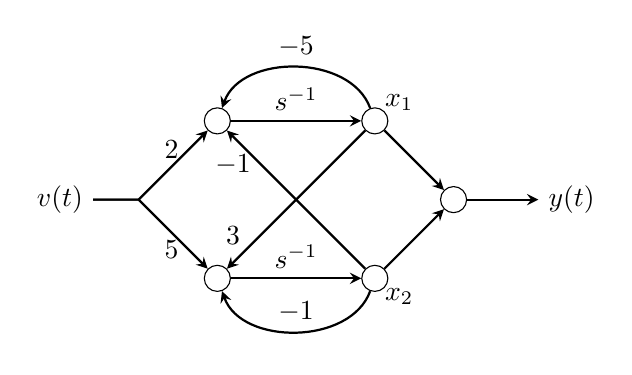
\begin{tikzpicture}[auto,>=stealth,thick]
\tikzstyle{unit}=[circle,draw,thin,fill=white,minimum width=.1pt,minimum height=.1pt]
  \node(x)at(0,0)[]{$v(t)$};
  \node(in1)at(2,1)[unit]{};
  \node(in2)at(2,-1)[unit]{};
  \node(x1)at(4,1)[unit]{};
  \node(x2)at(4,-1)[unit]{};
  \node(out)at(5,0)[unit]{};
  \node(y)at(6.5,0)[]{$y(t)$};
  \draw[->](x)--(1,0)--node[left,shift={(.2,.2)}]{$2$}(in1);
  \draw[->](in1)--node[]{$s^{-1}$}(x1);
  \draw[->](x1)to[out=110,in=70]node[above]{$-5$}(in1);
  \draw[->](x1)--(in2)node[above,shift={(.2,.3)}]{$3$};
  \draw[->](x1)--(out);
  \draw[->](x)--(1,0)--node[left,shift={(.2,-.2)}]{$5$}(in2);
  \draw[->](in2)--node[]{$s^{-1}$}(x2);
  \draw[->](x2)to[out=250,in=290]node[above]{$-1$}(in2);
  \draw[->](x2)--(in1)node[below,shift={(.2,-.3)}]{$-1$};
  \draw[->](x2)--(out);
  \draw[->](out)--(y);
  \draw[shift={(4,1)}](0pt,0pt)--(0pt,0pt) node[above right]{$x_1$};
  \draw[shift={(4,-1)}](0pt,0pt)--(0pt,0pt) node[below right]{$x_2$};
\end{tikzpicture}
\end{minipage}










\end{CJK}
\end{spacing}
\end{document}
